\documentclass[10pt]{article}
\usepackage[a4paper,margin=2cm]{geometry}
\usepackage{xeCJK}\setCJKmainfont{Microsoft JhengHei}\xeCJKsetup{CJKecglue={}}
\usepackage{booktabs,graphicx,amsmath,float,caption,hyperref,xcolor}
\hypersetup{colorlinks=true,linkcolor=blue!50!black,urlcolor=blue!50!black}
\graphicspath{{../figs/}}
\captionsetup{font=small}
\setlength{\parskip}{4pt}\setlength{\parindent}{0pt}
\def\tabbaseline{%
baseline\_val16 & 10 & 97.3 & 93.8 & +3.6 & 0.197 & 81.9 & 96.7 & 57.3 & 92.2 \\
baseline\_s0 & 10 & 97.2 & 95.3 & +1.9 & 0.123 & 80.8 & 95.6 & 56.0 & 90.9 \\
baseline\_s1 & 10 & 96.7 & 95.6 & +1.0 & 0.140 & 83.5 & 90.5 & 71.8 & 91.1 \\
baseline\_s2 & 10 & 96.3 & 95.3 & +1.0 & 0.142 & 77.2 & 96.4 & 45.3 & 88.5 \\}
\def\tablr{%
lr\_0.0001 & 8 & 95.1 & 96.3 & +10.9 & 0.283 & 80.8 & 94.6 & 57.7 & 91.3 \\
lr\_0.001 & 10 & 97.2 & 95.3 & +1.9 & 0.123 & 80.8 & 95.6 & 56.0 & 90.9 \\
lr\_0.01 & 4 & 94.7 & 93.6 & +2.5 & 0.189 & 80.9 & 89.2 & 67.1 & 90.6 \\}
\def\tabbs{%
bs\_16 & 10 & 95.8 & 95.6 & +0.2 & 0.105 & 83.0 & 94.9 & 63.2 & 92.1 \\
bs\_64 & 10 & 97.2 & 95.3 & +1.9 & 0.123 & 80.8 & 95.6 & 56.0 & 90.9 \\
bs\_256 & 10 & 95.7 & 95.6 & +0.1 & 0.174 & 82.5 & 93.1 & 65.0 & 92.8 \\}
\def\tabopt{%
opt\_sgd & 10 & 94.6 & 95.6 & $-$1.0 & 0.206 & 79.2 & 96.4 & 50.4 & 91.3 \\
opt\_sgdm & 10 & 97.1 & 95.6 & +1.5 & 0.120 & 81.9 & 95.9 & 58.5 & 91.8 \\
opt\_adam & 10 & 97.2 & 95.3 & +1.9 & 0.123 & 80.8 & 95.6 & 56.0 & 90.9 \\
opt\_adamw & 5 & 97.7 & 96.0 & +23.6 & 0.131 & 82.5 & 95.1 & 61.5 & 92.0 \\}
\def\tabsched{%
sched\_none & 29 & 97.4 & 95.6 & +4.1 & 0.171 & 84.6 & 92.1 & 72.2 & 92.9 \\
sched\_step & 23 & 99.1 & 96.3 & +3.2 & 0.117 & 82.2 & 96.7 & 58.1 & 91.2 \\
sched\_cosine & 30 & 99.5 & 95.6 & +3.8 & 0.134 & 81.1 & 96.9 & 54.7 & 90.9 \\
sched\_plateau & 23 & 98.8 & 95.6 & +3.5 & 0.116 & 81.2 & 96.7 & 55.6 & 91.1 \\}
\def\tabepochs{%
ep\_5 & 4 & 95.3 & 95.3 & +0.4 & 0.153 & 82.2 & 96.2 & 59.0 & 92.1 \\
ep\_10 & 4 & 96.9 & 95.3 & +22.1 & 0.153 & 82.2 & 96.2 & 59.0 & 92.1 \\
ep\_30 (= sched\_none) & 29 & 97.4 & 95.6 & +4.1 & 0.171 & 84.6 & 92.1 & 72.2 & 92.9 \\
ep\_60 & 53 & 96.8 & 95.6 & +5.2 & 0.138 & 81.2 & 96.7 & 55.6 & 89.2 \\}
\def\tabwd{%
wd\_0 & 17 & 99.5 & 96.6 & +4.5 & 0.134 & 84.5 & 92.8 & 70.5 & 92.8 \\
wd\_0.0001 & 18 & 99.5 & 96.3 & +4.5 & 0.130 & 81.4 & 91.0 & 65.4 & 90.8 \\
wd\_0.001 & 30 & 99.5 & 95.6 & +3.8 & 0.134 & 81.1 & 96.9 & 54.7 & 90.9 \\
wd\_0.01 & 29 & 99.4 & 96.3 & +3.8 & 0.127 & 79.6 & 98.5 & 48.3 & 89.5 \\
wd\_0.1 & 30 & 98.5 & 96.3 & +2.2 & 0.145 & 80.9 & 97.7 & 53.0 & 90.7 \\}
\def\tabarch{%
mlp\_d1\_w64 & 6 & 99.3 & 96.0 & +3.7 & 0.132 & 82.7 & 94.1 & 63.7 & 92.3 \\
mlp\_d3\_w64 & 19 & 98.9 & 96.0 & +3.7 & 0.109 & 82.1 & 97.2 & 56.8 & 91.5 \\
mlp\_d5\_w64 & 19 & 97.5 & 96.0 & +1.9 & 0.123 & 82.5 & 94.6 & 62.4 & 92.2 \\
mlp\_d3\_w256 & 20 & 99.7 & 96.3 & +3.4 & 0.113 & 79.5 & 97.4 & 49.6 & 91.6 \\
mlp\_d3\_w64\_nodrop & 19 & 100.0 & 96.3 & +4.0 & 0.117 & 81.9 & 96.9 & 56.8 & 88.8 \\
mlp\_d3\_w64\_nobn & 18 & 74.0 & 95.3 & $-$20.9 & 0.401 & 82.7 & 91.5 & 67.9 & 86.1 \\
cnn & 20 & 100.0 & 98.3 & +1.7 & 0.044 & 81.1 & 99.0 & 51.3 & 94.1 \\
cnn\_nodrop & 20 & 100.0 & 98.0 & +2.0 & 0.043 & 80.4 & 98.7 & 50.0 & 94.4 \\
cnn\_nobn & 16 & 91.5 & 91.6 & +1.0 & 0.243 & 85.3 & 87.7 & 81.2 & 92.1 \\
cnn\_narrow & 18 & 99.9 & 98.0 & +2.0 & 0.049 & 80.3 & 98.5 & 50.0 & 93.7 \\}
\def\tabaug{%
aug\_none & 20 & 100.0 & 98.3 & +1.7 & 0.044 & 81.1 & 99.0 & 51.3 & 94.1 \\
aug\_hflip & 20 & 99.9 & 98.7 & +1.2 & 0.051 & 80.3 & 99.0 & 49.1 & 93.5 \\
aug\_rot10 & 20 & 99.5 & 98.0 & +1.6 & 0.057 & 83.8 & 98.7 & 59.0 & 94.7 \\
aug\_affine & 17 & 98.9 & 98.3 & +0.9 & 0.054 & 85.1 & 98.2 & 63.2 & 95.5 \\
aug\_crop & 16 & 98.6 & 97.6 & +0.9 & 0.068 & 84.9 & 99.2 & 61.1 & 95.9 \\
aug\_bc & 16 & 99.9 & 98.0 & +2.3 & 0.050 & 80.8 & 98.7 & 50.9 & 94.6 \\
aug\_medical & 20 & 98.4 & 98.3 & +0.1 & 0.065 & 88.9 & 97.9 & 73.9 & 96.3 \\
aug\_autoaug & 6 & 97.9 & 98.0 & +0.6 & 0.086 & 82.4 & 97.7 & 56.8 & 93.4 \\
aug\_randaug & 18 & 98.4 & 98.7 & +0.4 & 0.048 & 83.5 & 98.5 & 58.5 & 95.6 \\
aug\_trivial & 16 & 97.3 & 98.7 & $-$1.0 & 0.059 & 82.7 & 99.0 & 55.6 & 95.6 \\
aug\_vflip\_rot90 & 20 & 99.1 & 96.6 & +2.4 & 0.071 & 81.6 & 99.0 & 52.6 & 94.4 \\}
\def\tabfinal{%
final\_s0 & 20 & 98.9 & 98.7 & +1.0 & 0.053 & 83.2 & 98.7 & 57.3 & 95.6 \\
final\_s1 & 30 & 98.5 & 98.3 & +0.2 & 0.052 & 83.8 & 99.0 & 58.5 & 95.5 \\
final\_s2 & 17 & 98.8 & 98.7 & +0.5 & 0.046 & 88.0 & 97.9 & 71.4 & 96.2 \\}
\def\tabsummary{%
baseline\_s0 & 10 & 97.2 & 95.3 & +1.9 & 0.123 & 80.8 & 95.6 & 56.0 & 90.9 \\
lr\_0.01 & 4 & 94.7 & 93.6 & +2.5 & 0.189 & 80.9 & 89.2 & 67.1 & 90.6 \\
opt\_sgd & 10 & 94.6 & 95.6 & $-$1.0 & 0.206 & 79.2 & 96.4 & 50.4 & 91.3 \\
sched\_none & 29 & 97.4 & 95.6 & +4.1 & 0.171 & 84.6 & 92.1 & 72.2 & 92.9 \\
sched\_step & 23 & 99.1 & 96.3 & +3.2 & 0.117 & 82.2 & 96.7 & 58.1 & 91.2 \\
wd\_0.1 & 30 & 98.5 & 96.3 & +2.2 & 0.145 & 80.9 & 97.7 & 53.0 & 90.7 \\
mlp\_d3\_w256 & 20 & 99.7 & 96.3 & +3.4 & 0.113 & 79.5 & 97.4 & 49.6 & 91.6 \\
cnn & 20 & 100.0 & 98.3 & +1.7 & 0.044 & 81.1 & 99.0 & 51.3 & 94.1 \\
cnn\_nobn & 16 & 91.5 & 91.6 & +1.0 & 0.243 & 85.3 & 87.7 & 81.2 & 92.1 \\
aug\_bc & 16 & 99.9 & 98.0 & +2.3 & 0.050 & 80.8 & 98.7 & 50.9 & 94.6 \\
aug\_affine & 17 & 98.9 & 98.3 & +0.9 & 0.054 & 85.1 & 98.2 & 63.2 & 95.5 \\
aug\_medical & 20 & 98.4 & 98.3 & +0.1 & 0.065 & 88.9 & 97.9 & 73.9 & 96.3 \\
aug\_randaug & 18 & 98.4 & 98.7 & +0.4 & 0.048 & 83.5 & 98.5 & 58.5 & 95.6 \\
aug\_vflip\_rot90 & 20 & 99.1 & 96.6 & +2.4 & 0.071 & 81.6 & 99.0 & 52.6 & 94.4 \\
final\_s0 & 20 & 98.9 & 98.7 & +1.0 & 0.053 & 83.2 & 98.7 & 57.3 & 95.6 \\
final\_s1 & 30 & 98.5 & 98.3 & +0.2 & 0.052 & 83.8 & 99.0 & 58.5 & 95.5 \\
final\_s2 & 17 & 98.8 & 98.7 & +0.5 & 0.046 & 88.0 & 97.9 & 71.4 & 96.2 \\}

\newcommand{\baseacc}{80.5 $\pm$ 3.1}
\newcommand{\finalacc}{85.0 $\pm$ 2.6}
\newcommand{\basesens}{94.2 $\pm$ 3.2}
\newcommand{\finalsens}{98.5 $\pm$ 0.5}
\newcommand{\basespec}{57.7 $\pm$ 13.3}
\newcommand{\finalspec}{62.4 $\pm$ 7.8}
\newcommand{\baseauc}{90.1 $\pm$ 1.5}
\newcommand{\finalauc}{95.8 $\pm$ 0.4}
\newcommand{\basevalacc}{95.4 $\pm$ 0.2}
\newcommand{\finalvalacc}{98.5 $\pm$ 0.2}
\newcommand{\finalcfg}{aug\_randaug}

\newcommand{\thead}{run & best ep & train acc & val acc & gap & val loss & test acc & sens & spec & AUC \\ \midrule}
\newcommand{\rtab}[2]{\begin{table}[H]\centering\small\caption{#2}\begin{tabular}{lrrrrrrrrr}\toprule\thead #1 \bottomrule\end{tabular}\end{table}}

\title{HW3: Hyperparameter Tuning --- Chest X-ray Pneumonia Classification\\\large Deep Learning in Biomedical Optical Imaging (11510IPT 553000)}
\author{115061534 江承瀚}
\date{}
\begin{document}
\maketitle

\paragraph{Setup and conventions.}
All experiments use the provided starter code with three fixes (Section~1.3) and run on CPU (PyTorch 2.11).
Images are resized to $256\times256$ (bicubic) and converted to one gray channel, as in the starter.
In every table, \emph{train acc} and \emph{gap} (= train acc $-$ val acc) are from the \textbf{last} epoch.
\emph{val acc}, \emph{val loss} and all test metrics are from the checkpoint with the best validation accuracy.
\emph{sens} = sensitivity (recall of PNEUMONIA), \emph{spec} = specificity (recall of NORMAL). The threshold is 0.5.
All numbers are percentages, except epochs and loss.
Unless stated otherwise, a run uses one seed (0) and changes one factor from the reference configuration.
The code (\texttt{115061534\_江承瀚\_HW3.ipynb}) writes every result to \texttt{results/*.json}.
The script \texttt{report/make\_tables.py} builds all tables in this report from those files, so no number is copied by hand.

%==============================================================
\section{Data \& Baseline Analysis}
\subsection{Class distribution and splits}
\begin{table}[H]\centering\small
\caption{Images per split. The course version of the dataset is a balanced subset of the Kermany chest X-ray set.}
\begin{tabular}{lrrrrl}\toprule
split & NORMAL & PNEUMONIA (bacteria / virus) & total & \% PNEU & patients\\\midrule
train (official) & 1000 & 1000 (708 / 292) & 2000 & 50.0 & 1201\\
val (official) & 8 & 8 (8 / 0) & 16 & 50.0 & 15\\
test (official) & 234 & 390 (242 / 148) & 624 & 62.5 & 427\\\midrule
train-split (ours) & \multicolumn{4}{l}{85\,\% of the training patients of each class} & \\
val-split (ours) & \multicolumn{4}{l}{15\,\% of the training patients of each class (297 images, see notebook)} & \\
\bottomrule\end{tabular}\end{table}

\begin{figure}[H]\centering
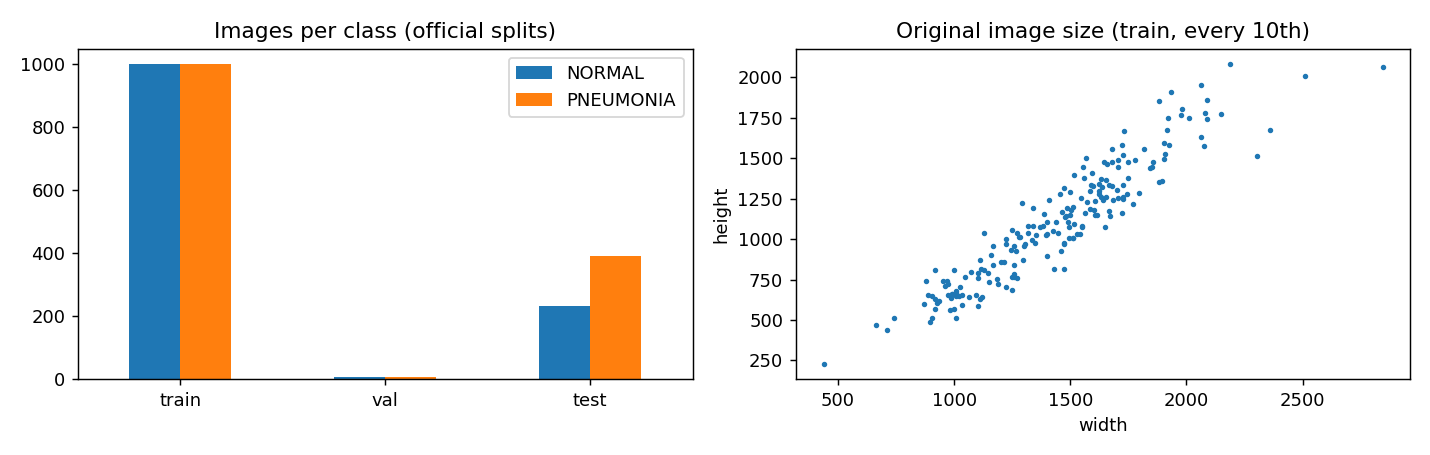
\includegraphics[width=.75\linewidth]{s1_class_dist.png}\\
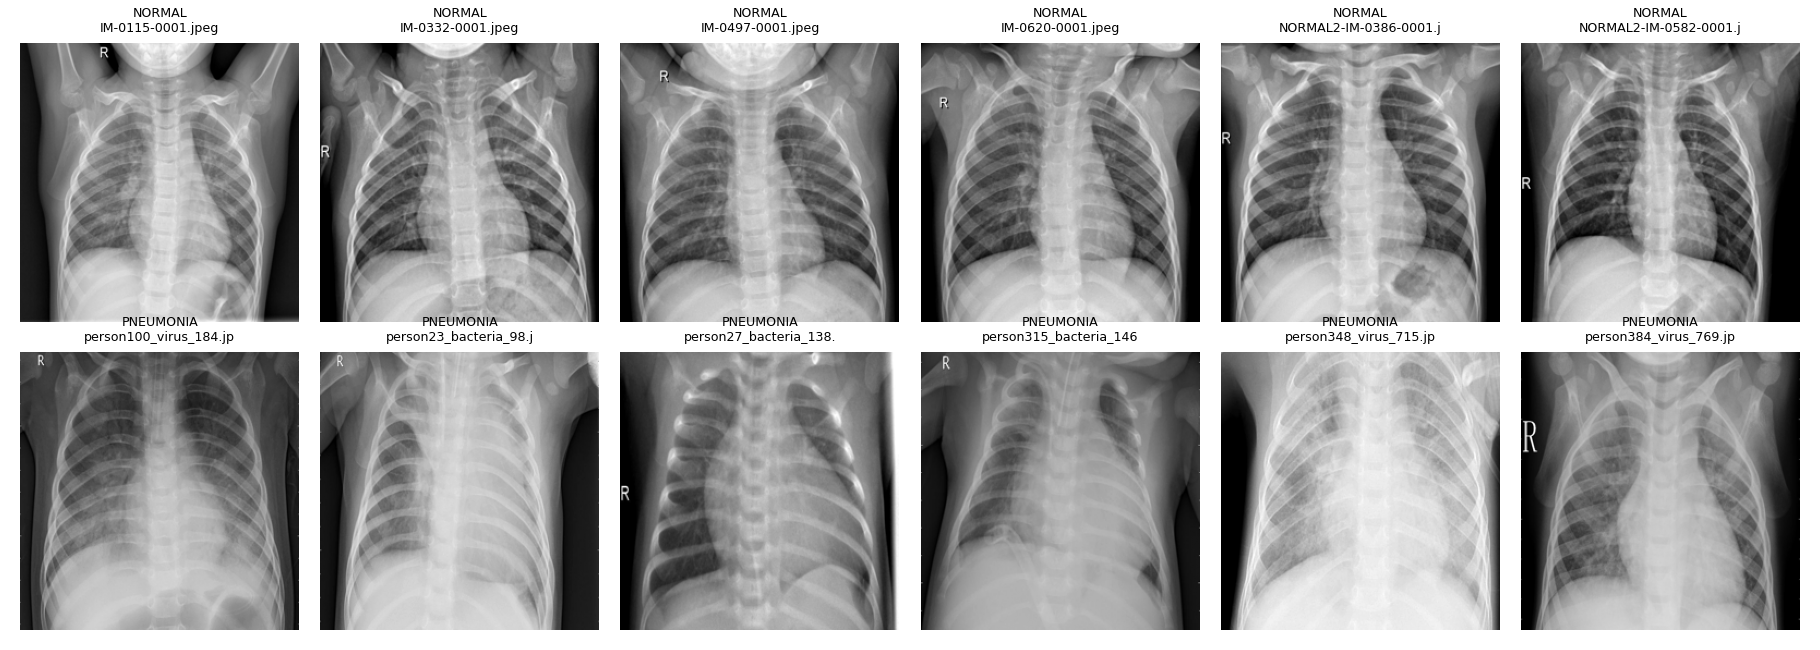
\includegraphics[width=.85\linewidth]{s1_samples.png}
\caption{Top: class counts and the original image sizes (445--2534 px wide, mixed aspect ratios, 5\,\% RGB). Bottom: training examples after the $256\times256$ resize.}
\end{figure}

Observations:
\begin{itemize}
\item \textbf{The training set is balanced, but the test set is not.} The training set is 50/50. The test set is 62.5\,\% PNEUMONIA.
  A model that predicts ``PNEUMONIA'' for every image gets 62.5\,\% test accuracy. This value is the floor for test accuracy.
  Accuracy alone also hides the trade-off between sensitivity and specificity, so I also report sensitivity, specificity and ROC-AUC.
\item \textbf{The PNEUMONIA class has two subtypes.} Viral pneumonia is 29\,\% of the training PNEUMONIA images but 38\,\% of the test PNEUMONIA images.
  The official validation set has no viral images at all.
\item \textbf{One patient can have many images.} The 2000 training images come from 1201 patients (up to 30 images for one patient).
  If we split by image, images of the same patient go to both training and validation, and the validation score is too high.
\item \textbf{The image sizes vary.} The resize to a square changes the aspect ratio of most images (the median original size is about $1360\times990$).
  The images also have different exposure and contrast, and some contain text markers (for example the ``R'' marker).
\end{itemize}

\subsection{Is the official validation set reliable?}
No. The official validation set has 16 images, so one image changes the accuracy by 6.25 points.
The binomial standard error of an accuracy near 85\,\% is $\sqrt{0.85\cdot0.15/16}=8.9$ points with 16 images.
With our 297-image val-split, the standard error is 2.1 points.
In our runs, the 16-image accuracy of the selected checkpoints is between 62.5\,\% and 100\,\% for models whose test accuracy differs by only a few points (column \texttt{val16} in \texttt{results/}).
The 16 images also contain no viral pneumonia, and the curves in Figure~\ref{fig:base} jump by steps of 6.25 points.
For this reason, I made a \textbf{patient-grouped, class-stratified val-split} from the training set (15\,\% of the patients of each class).
I use it for checkpoint selection and model selection in all later experiments.
The official 16 images are still evaluated and stored.

\subsection{Baseline}
Fixes to the starter code:
(1) the starter created \texttt{lr\_scheduler} before \texttt{optimizer}, which raises a \texttt{NameError}, so I create the scheduler after the optimizer;
(2) the starter averaged per-batch accuracies, which gives the last (smaller) batch too much weight, so I compute accuracy over the whole set;
(3) the starter evaluated with a global \texttt{criterion}. I use one \texttt{metrics()} function for validation and test.
The baseline is the starter MLP ($65536\to64\to64\to64\to1$, BatchNorm, ReLU, Dropout 0.5, 4.2\,M parameters) trained with Adam (lr $10^{-3}$, weight decay $10^{-3}$), batch size 64, ReduceLROnPlateau and 10 epochs.

\rtab{\tabbaseline}{Baseline. \texttt{baseline\_val16}: the original protocol (all 2000 training images, checkpoint selected on the 16 official images). \texttt{baseline\_s0..2}: the reference protocol (train-split / val-split) with 3 seeds.}

\begin{figure}[H]\centering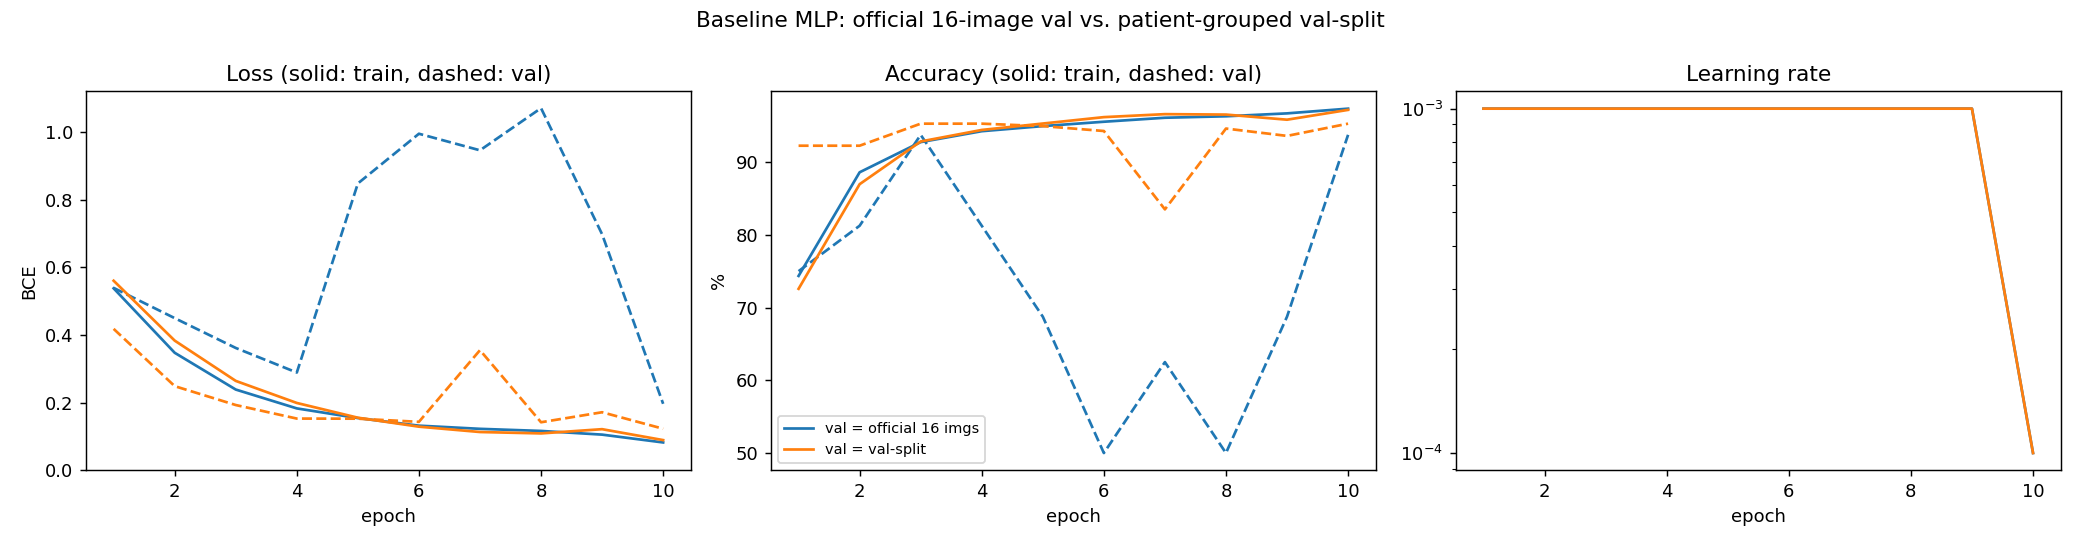
\includegraphics[width=\linewidth]{s1_baseline.png}
\caption{Baseline learning curves (solid lines: train, dashed lines: validation). The 16-image validation curve moves in steps of 6.25 points.}\label{fig:base}\end{figure}

\textbf{Results.} The baseline reaches about 95\,\% validation accuracy, but its test accuracy is only \baseacc\ (mean $\pm$ std over 3 seeds).
Sensitivity is \basesens, specificity is \basespec, and AUC is \baseauc.
\begin{itemize}
\item \textbf{The test set differs from the training data.} Validation accuracy (images from the training distribution) is 12--15 points higher than test accuracy.
 Almost all test errors are false positives: NORMAL test images classified as PNEUMONIA.
 The model has learned features that do not transfer well to the test images.
\item \textbf{Seed variation is large.} With the same configuration, only the seed changes the test accuracy by about 6 points and the specificity by more than 20 points.
 For this reason, I treat a single-seed difference of a few points as not significant in Sections 2--5.
\end{itemize}

%==============================================================
\section{Optimization Settings}
Reference: the baseline MLP, 10 epochs, weight decay $10^{-3}$, ReduceLROnPlateau, val-split, seed 0. I change one factor at a time.

\rtab{\tablr}{Learning rate (Adam, batch size 64).}
\begin{figure}[H]\centering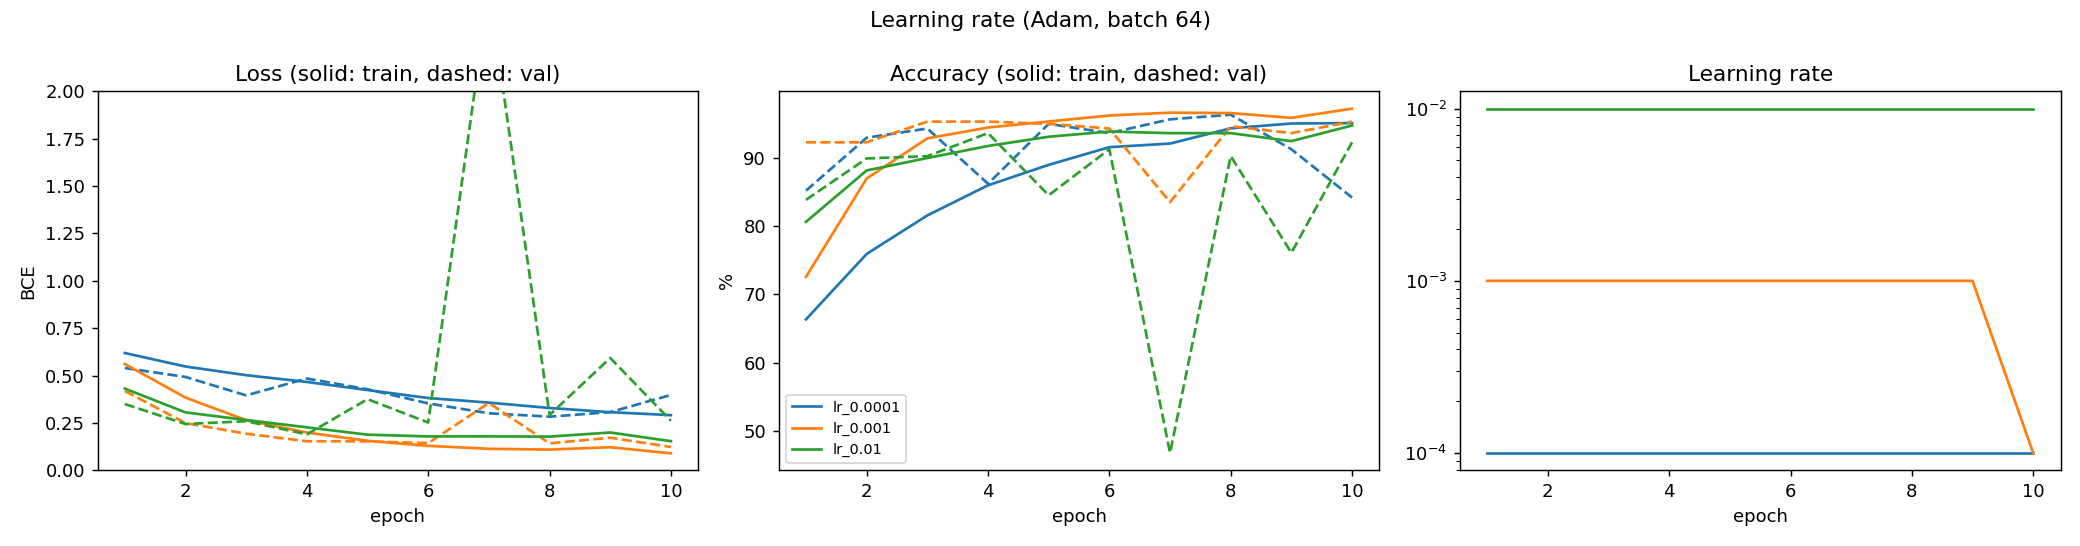
\includegraphics[width=\linewidth]{s2_lr.png}\caption{Learning rate.}\end{figure}
\textbf{Learning rate.} The learning rate controls both convergence speed and stability.
With lr $10^{-4}$ the training loss decreases slowly (0.62 $\rightarrow$ 0.29 in 10 epochs), so the model underfits within this budget.
With lr $10^{-3}$ the training loss reaches about 0.1, and the validation curve is mostly stable.
With lr $10^{-2}$ the training loss does not go below about 0.15, and the validation loss spikes to 2.5 at epoch 7 (validation accuracy falls to 47\,\%, which is a one-class output).
The updates are too large for the first layer, which has 4.2\,M weights. They also disturb the BatchNorm statistics, so the model jumps between states.
The best checkpoint of lr $10^{-2}$ is at epoch 4, before the oscillation starts.
The test accuracy of the three runs is almost the same (about 81\,\%). This is because checkpoint selection picks a good epoch in every run, and because the error on the shifted test set is dominated by specificity, not by optimization.
Conclusion: $10^{-3}$ gives the best balance for Adam. $10^{-2}$ is unstable, and $10^{-4}$ needs more epochs.

\rtab{\tabbs}{Batch size (Adam, lr $10^{-3}$).}
\begin{figure}[H]\centering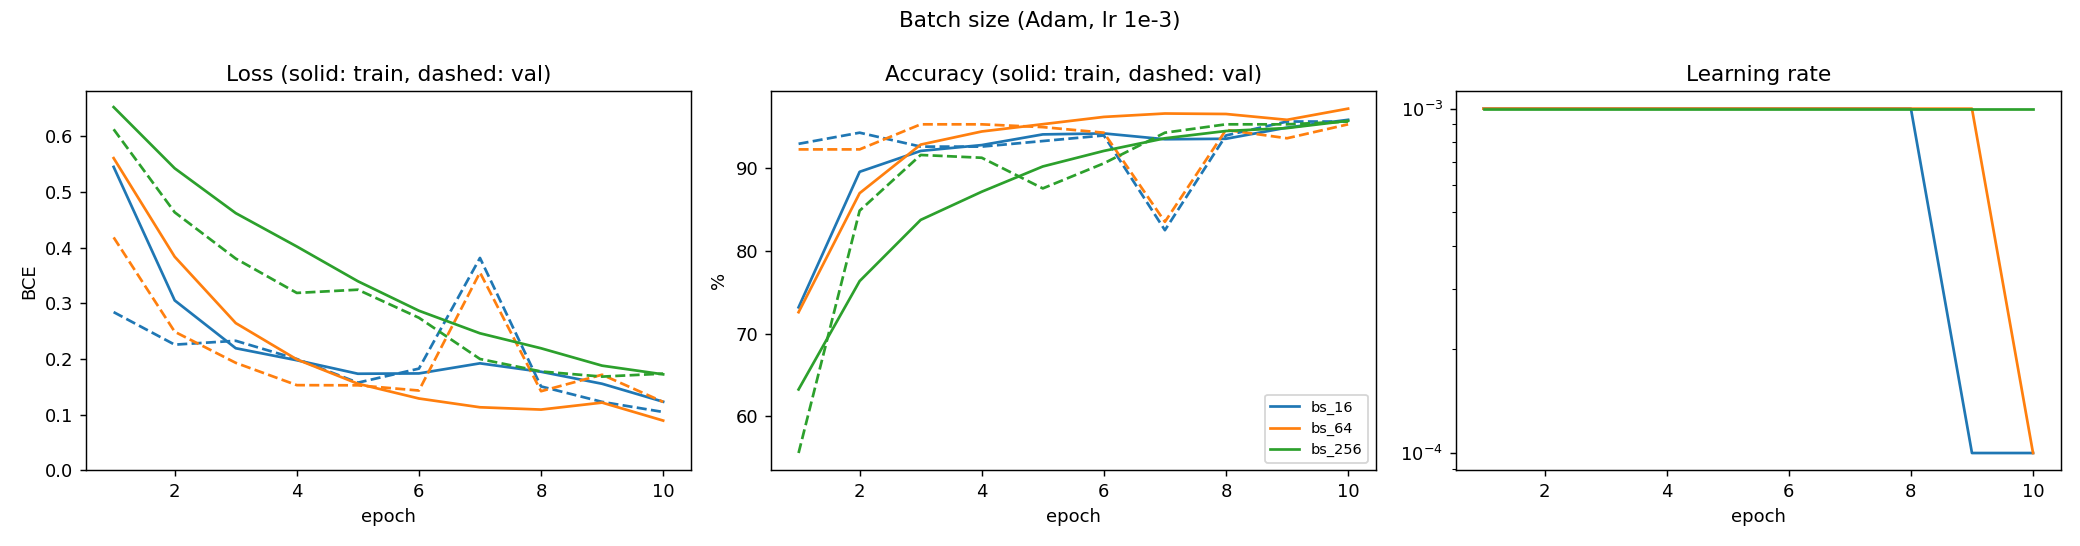
\includegraphics[width=\linewidth]{s2_bs.png}\caption{Batch size.}\end{figure}
\textbf{Batch size.} With a fixed number of epochs, a smaller batch size gives more updates per epoch (107 updates with batch size 16, 27 with 64, 7 with 256), and each gradient is noisier.
Batch size 256 converges slowest. Its validation accuracy is 56\,\% after the first epoch, and its training loss is still 0.17 at epoch 10. With the same learning rate, it simply takes fewer steps.
Its curves are the smoothest, because each gradient is averaged over more samples.
Batch size 16 converges fastest per epoch, but its validation curve has a dip (82\,\% at epoch 7). Small, noisy batches also make the BatchNorm batch statistics less stable.
Batch size 16 costs about 1.6 times the wall-clock time per epoch on CPU (9.7\,s vs.\ 5.9\,s), because the batches are too small to use the hardware well.
The test results of all three batch sizes (80.8--83.0\,\%) are within the seed variation of the baseline.
Batch size 64 is a reasonable compromise. If we use batch size 256, we should scale the learning rate up (linear scaling rule) or train for more epochs.

\rtab{\tabopt}{Optimizer. SGD and SGD with momentum use lr $10^{-2}$. Adam and AdamW use lr $10^{-3}$. AdamW uses decoupled weight decay $10^{-2}$.}
\begin{figure}[H]\centering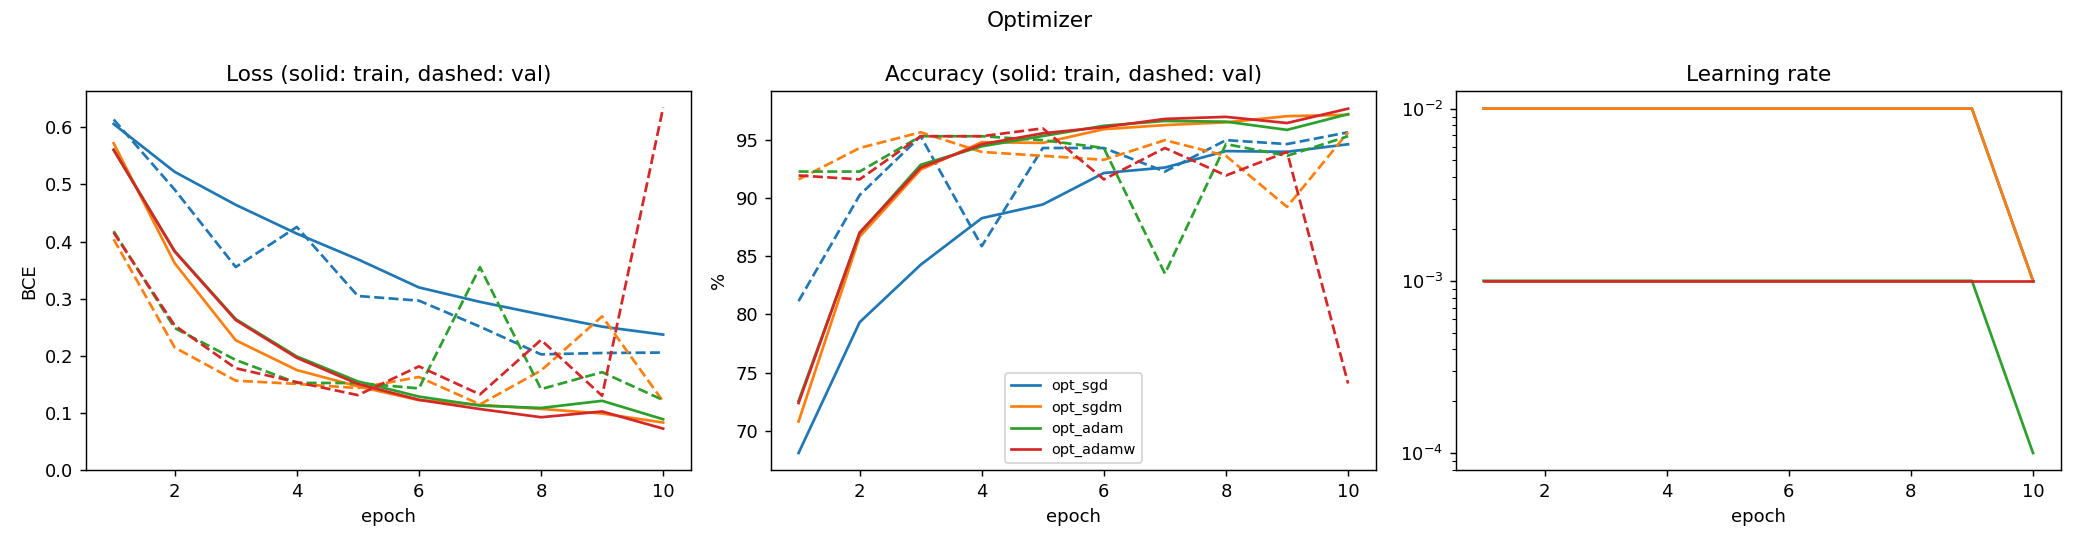
\includegraphics[width=\linewidth]{s2_opt.png}\caption{Optimizer.}\end{figure}
\textbf{Optimizer.} Plain SGD converges slowest (training loss 0.24 after 10 epochs, compared with about 0.08 for the others).
With momentum, SGD accumulates a velocity along directions where the gradient is consistent, so its speed is close to Adam's.
Adam and AdamW scale each parameter's step by a running estimate of the gradient magnitude.
This helps the first layer, whose 65\,536 inputs per unit get gradients of very different magnitudes.
Adam and AdamW reach the lowest training loss in the fewest epochs.
AdamW differs from Adam only in its decoupled weight decay. Its validation accuracy drops to 74\,\% at the last epoch, which shows that the larger decay (lr $10^{-3}$ and decay $10^{-2}$) does not prevent the instability seen in the other runs.
SGD with momentum and AdamW reach the highest validation accuracy, but the differences are 0.3--0.7 points, which is about 1--2 images.
The final ranking in this experiment is decided mainly by convergence speed: SGD $<$ SGD with momentum $\approx$ Adam $\approx$ AdamW.

%==============================================================
\section{Training Schedule \& Regularization}
Reference: the baseline MLP, Adam lr $10^{-3}$, batch size 64, val-split, seed 0.

\rtab{\tabsched}{LR scheduler, 30 epochs. StepLR: $\times0.1$ every 10 epochs. Cosine: $T_{max}=30$. Plateau: $\times0.1$ after 5 epochs without improvement in val acc.}
\begin{figure}[H]\centering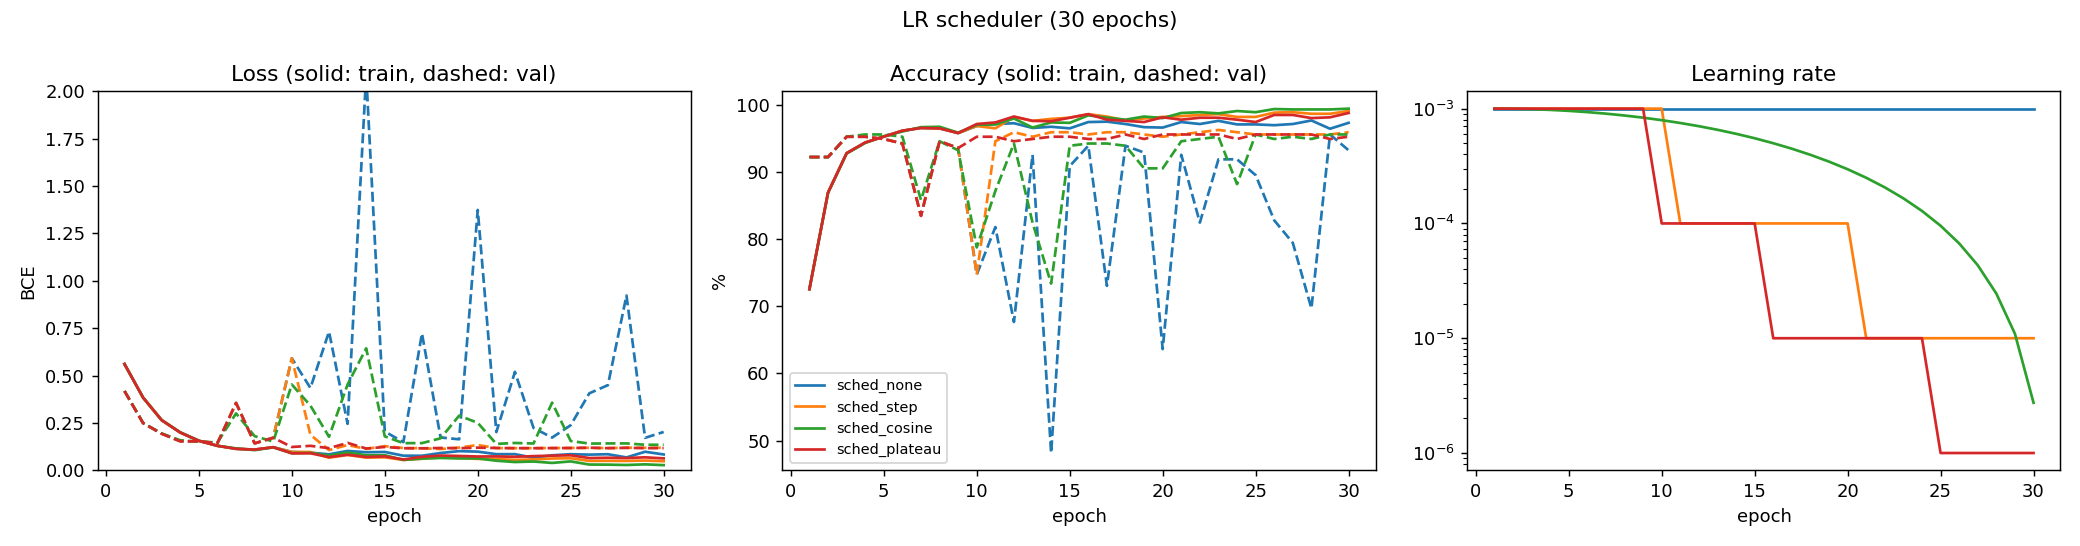
\includegraphics[width=\linewidth]{s3_sched.png}\caption{LR schedulers (the right panel shows the learning rate).}\end{figure}
\textbf{Scheduler.} All four runs are identical until epoch 10 (same seed). The differences come only from how the learning rate changes after that point.
Without a scheduler, the model keeps training at lr $10^{-3}$, and the validation accuracy oscillates strongly (from about 48 to 96\,\%), and the validation loss reaches 0.92 at epoch 28.
The training loss is near zero, so each large step moves the model to a different state.
StepLR ($\times0.1$ at epochs 10 and 20) and ReduceLROnPlateau both make the late epochs stable.
After the first learning-rate reduction, the validation accuracy stays at 95--96\,\% and the validation loss stays at 0.12.
Cosine annealing reduces the learning rate gradually, so its curve becomes stable later (after about epoch 20), but it reaches the lowest training loss (0.03).
The scheduler mainly affects the stability of late training. A scheduler lets us use a large learning rate early for fast progress and a small learning rate late for a stable result.
It does not change the best value found during training very much. Without a scheduler, a good epoch still exists, and the best-checkpoint selection finds it.
However, without a scheduler the final-epoch model is unreliable.

\rtab{\tabepochs}{Number of epochs (no scheduler, so the training length is the only change).}
\begin{figure}[H]\centering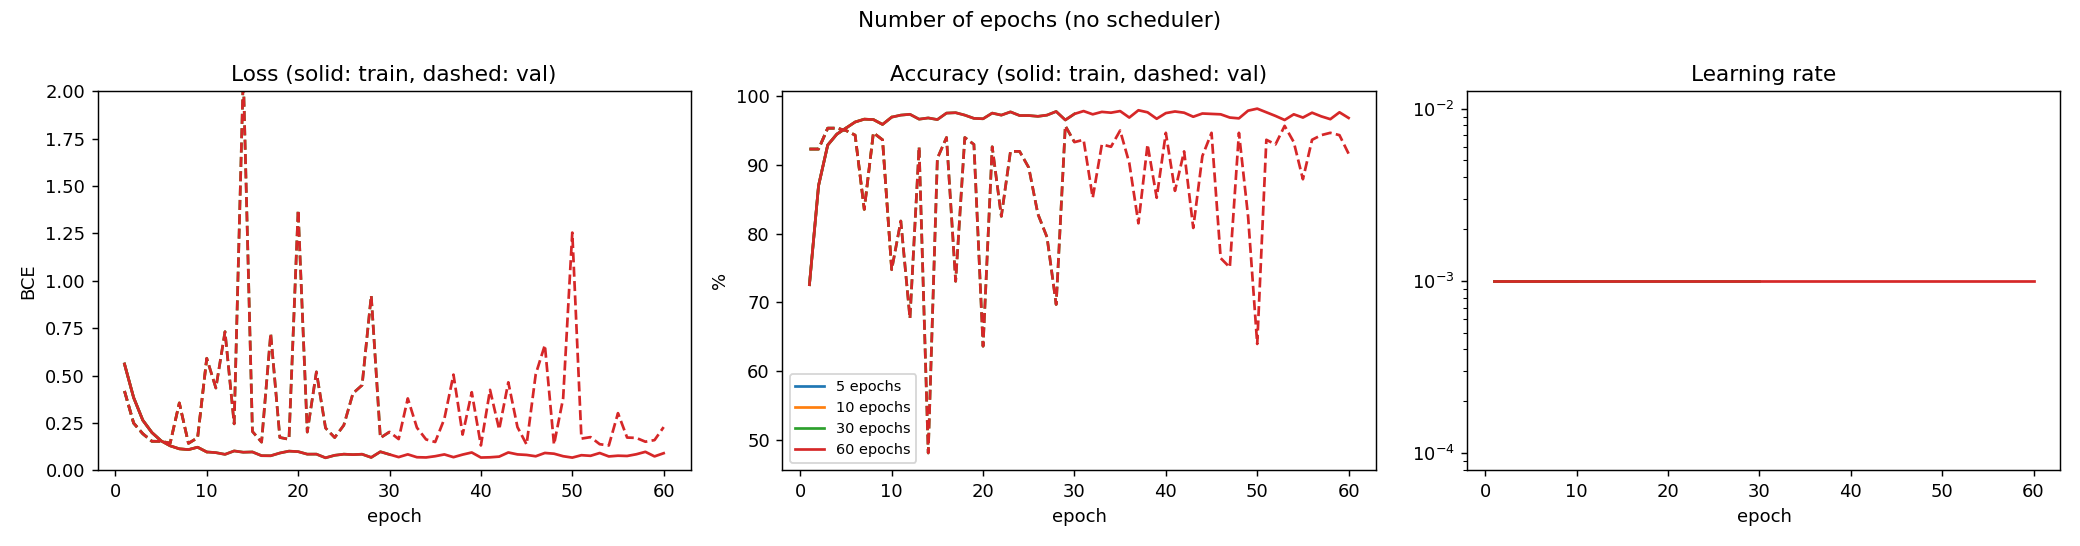
\includegraphics[width=\linewidth]{s3_epochs.png}\caption{Number of epochs. The runs use the same seed and no scheduler, so the shorter runs are prefixes of the 60-epoch run and their curves lie under it.}\end{figure}
\textbf{Epochs.} The 5-epoch and 10-epoch runs give the same model, because both select the checkpoint at epoch 4. The validation accuracy of this MLP saturates at about 95\,\% within 4--5 epochs.
Longer training without a scheduler does not help. The training accuracy stays at 96--97\,\% (dropout 0.5 limits it), the validation accuracy oscillates (it falls to 64\,\% around epoch 50), and the best epoch of the 60-epoch run (epoch 53) is no better on test than the 4-epoch run (81.2\,\% vs.\ 82.2\,\%, and AUC 89.2 vs.\ 92.1).
More epochs only add value when the learning rate also decreases (previous paragraph).
More epochs also give the checkpoint selection more chances to pick an epoch whose val-split score is high by chance, without a better test result.

\rtab{\tabwd}{Weight decay (Adam with an L2 term, 30 epochs, cosine schedule).}
\begin{figure}[H]\centering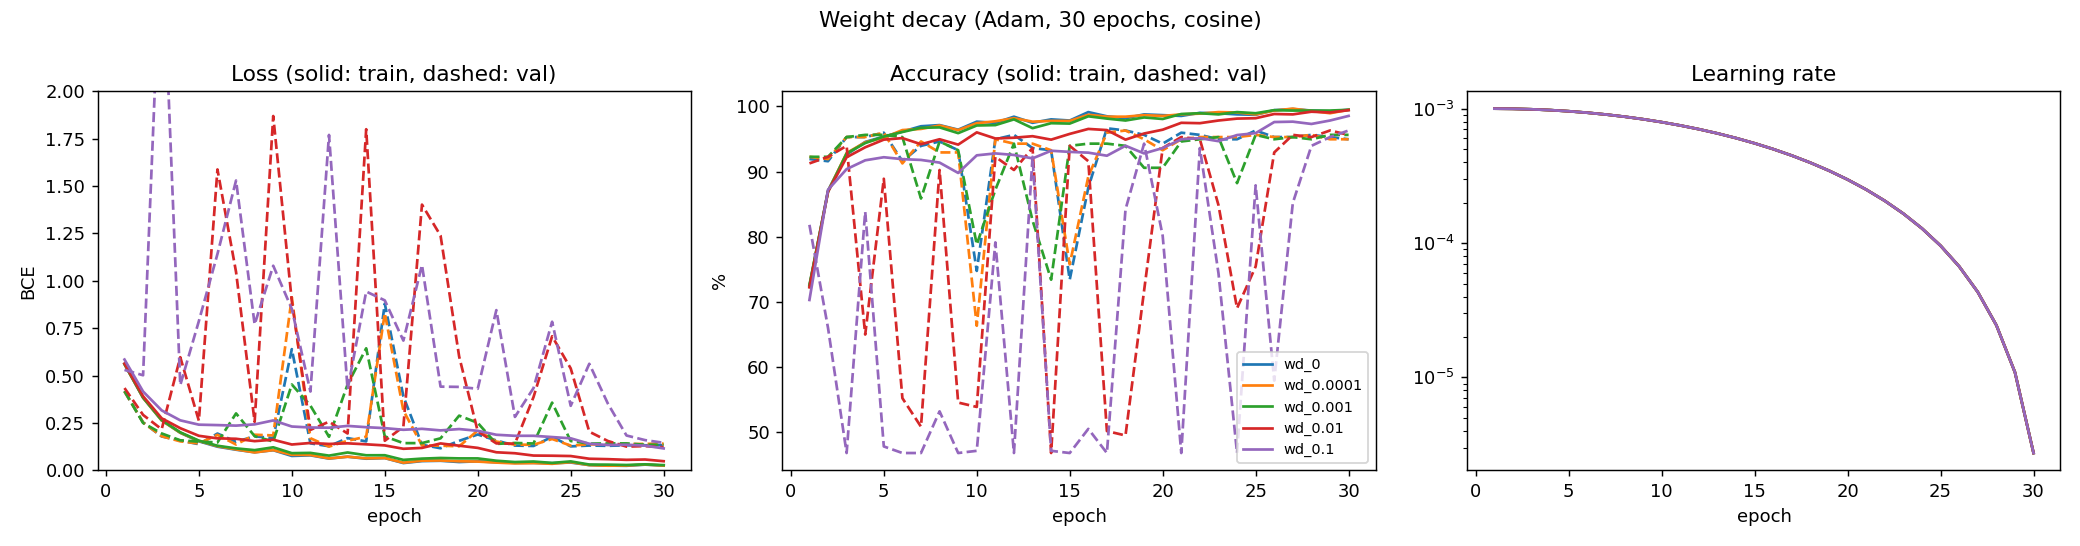
\includegraphics[width=\linewidth]{s3_wd.png}\caption{Weight decay.}\end{figure}
\textbf{Weight decay.} The decay values from 0 to $10^{-2}$ give almost the same curves. The final training loss is 0.02--0.05 and the train--val gap is about 3 points.
This is because, for this MLP, dropout 0.5 and BatchNorm already provide most of the regularization, and the L2 term inside Adam is divided by the adaptive denominator, which makes it weaker than in SGD.
With decay $10^{-1}$ the regularization is clearly too strong. The training loss stays high (0.12 at epoch 30), and the validation accuracy collapses to 47--51\,\% several times in the first half (BatchNorm on top of strongly shrunk weights).
The model recovers only after the cosine schedule reduces the learning rate.
On test, \texttt{wd\_0} has the highest single-seed score (84.5\,\%). However, this value is within the seed range of the baseline (77--84\,\%), and there is no monotonic trend.
Weight decay is therefore not an important factor here, except for the destabilizing value $10^{-1}$.

%==============================================================
\section{Model Architecture}
All runs: Adam lr $10^{-3}$, weight decay $10^{-3}$, batch size 64, cosine schedule, 20 epochs, seed 0.
\texttt{mlp\_d$k$\_w$n$} is an MLP with $k$ hidden layers of width $n$.
The CNN has a stride-2 $5\times5$ stem and four conv--BN--ReLU--maxpool blocks (16--32--64--128--128 channels), followed by global average pooling, dropout 0.3 and a linear layer (0.25\,M parameters).
\texttt{cnn\_narrow} halves all channel counts.

\rtab{\tabarch}{Architectures (params: MLP 4.2\,M, MLP w256 16.9\,M, CNN 0.25\,M, CNN narrow 0.06\,M).}
\begin{figure}[H]\centering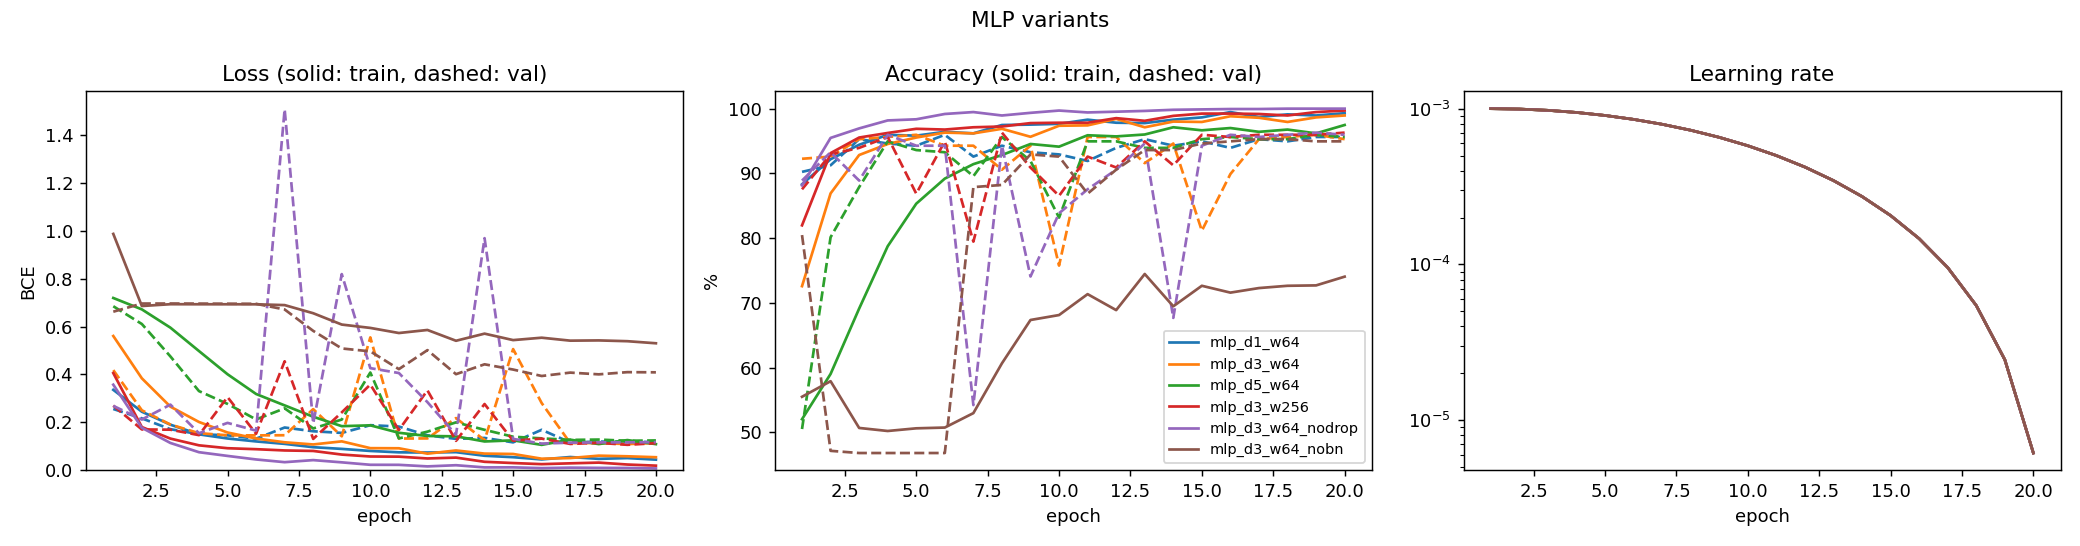
\includegraphics[width=\linewidth]{s4_mlp.png}\\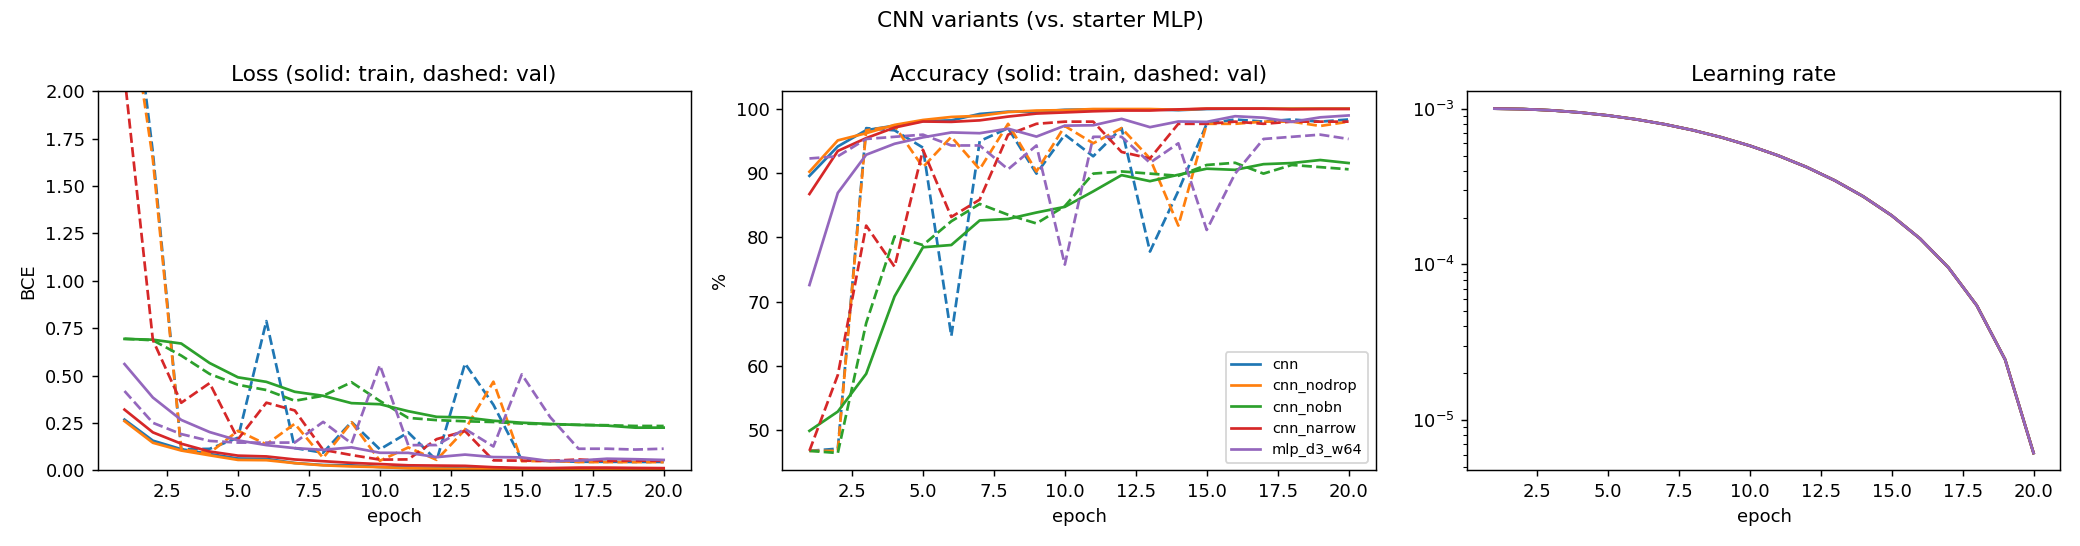
\includegraphics[width=\linewidth]{s4_cnn.png}
\caption{Top: MLP variants. Bottom: CNN variants compared with the starter MLP.}\end{figure}
\textbf{MLP depth and width.} All MLPs reach 96.0--96.3\,\% validation accuracy, and their test accuracy (79.5--82.7\,\%) is within the seed noise.
The MLP flattens the image, so it has no spatial prior. More than 99.9\,\% of its parameters are in the first $65536\times n$ layer, which learns one global template per hidden unit.
Extra depth (1 $\rightarrow$ 5 hidden layers of 64) does not add useful capacity. The 5-layer network trains more slowly (training loss 0.11 vs.\ 0.04), because there are more dropout layers in series.
Width 256 (16.9\,M parameters) fits the training set best (training loss 0.019) and has the lowest test specificity (49.6\,\%). This is the clearest overfitting among the MLPs: more capacity is used to memorize the training distribution.

\textbf{Dropout and normalization (MLP).} Without dropout, the training accuracy reaches 100\,\% (training loss 0.008), and the test AUC falls from 91.5 to 88.8. Dropout is the main regularizer of the MLP.
Without BatchNorm, the training accuracy measured with dropout active stays at 74\,\%, but the validation accuracy is still 95\,\%. Dropout 0.5 on unnormalized activations makes training noisy and slow.
The outputs are also less calibrated: the validation loss is 0.40 instead of 0.11, and the test AUC is the lowest (86.1).

\textbf{CNN vs.\ MLP.} The CNN has 17 times fewer parameters (0.25\,M) and is clearly better on the in-distribution data. Its validation accuracy is 98.3\,\% (vs.\ 96.0\,\%), its validation loss is 0.044 (vs.\ 0.109), and its test AUC is 94.1 (vs.\ 91.5).
Convolutions share weights over positions, and pooling gives some translation invariance. This prior fits the task: opacities can appear anywhere in the lung.
However, the CNN also fits the training set completely (training loss 0.004), and its test specificity at threshold 0.5 is 51\,\%. The higher test AUC shows that the CNN ranks the test images better.
At the 0.5 threshold, the CNN still classifies half of the NORMAL test images as PNEUMONIA, so its test accuracy (81.1\,\%) does not improve. This is overfitting to the training distribution, and Section 5 addresses it.
\texttt{cnn\_narrow} (0.06\,M parameters) is almost the same as \texttt{cnn}, so width is not the limiting factor.
Removing dropout from the CNN changes little (it already has BN and global pooling).
Removing BatchNorm from the CNN makes optimization much slower (training accuracy 91.5\,\%, validation 91.6\,\%), so the model underfits.
It also has the highest test accuracy and specificity of this group (85.3\,\% / 81.2\,\%), but a lower AUC (92.1).
The underfitted model gives less extreme probabilities, and this moves its operating point toward NORMAL. It does not rank the test images better.
For this reason, I compare models mainly by AUC and use accuracy at 0.5 with care.

%==============================================================
\section{Data Augmentation}
All runs: \texttt{cnn} (Section 4), Adam lr $10^{-3}$, weight decay $10^{-3}$, cosine schedule, 20 epochs, seed 0.
The augmentations are applied to the training images only.

\begin{figure}[H]\centering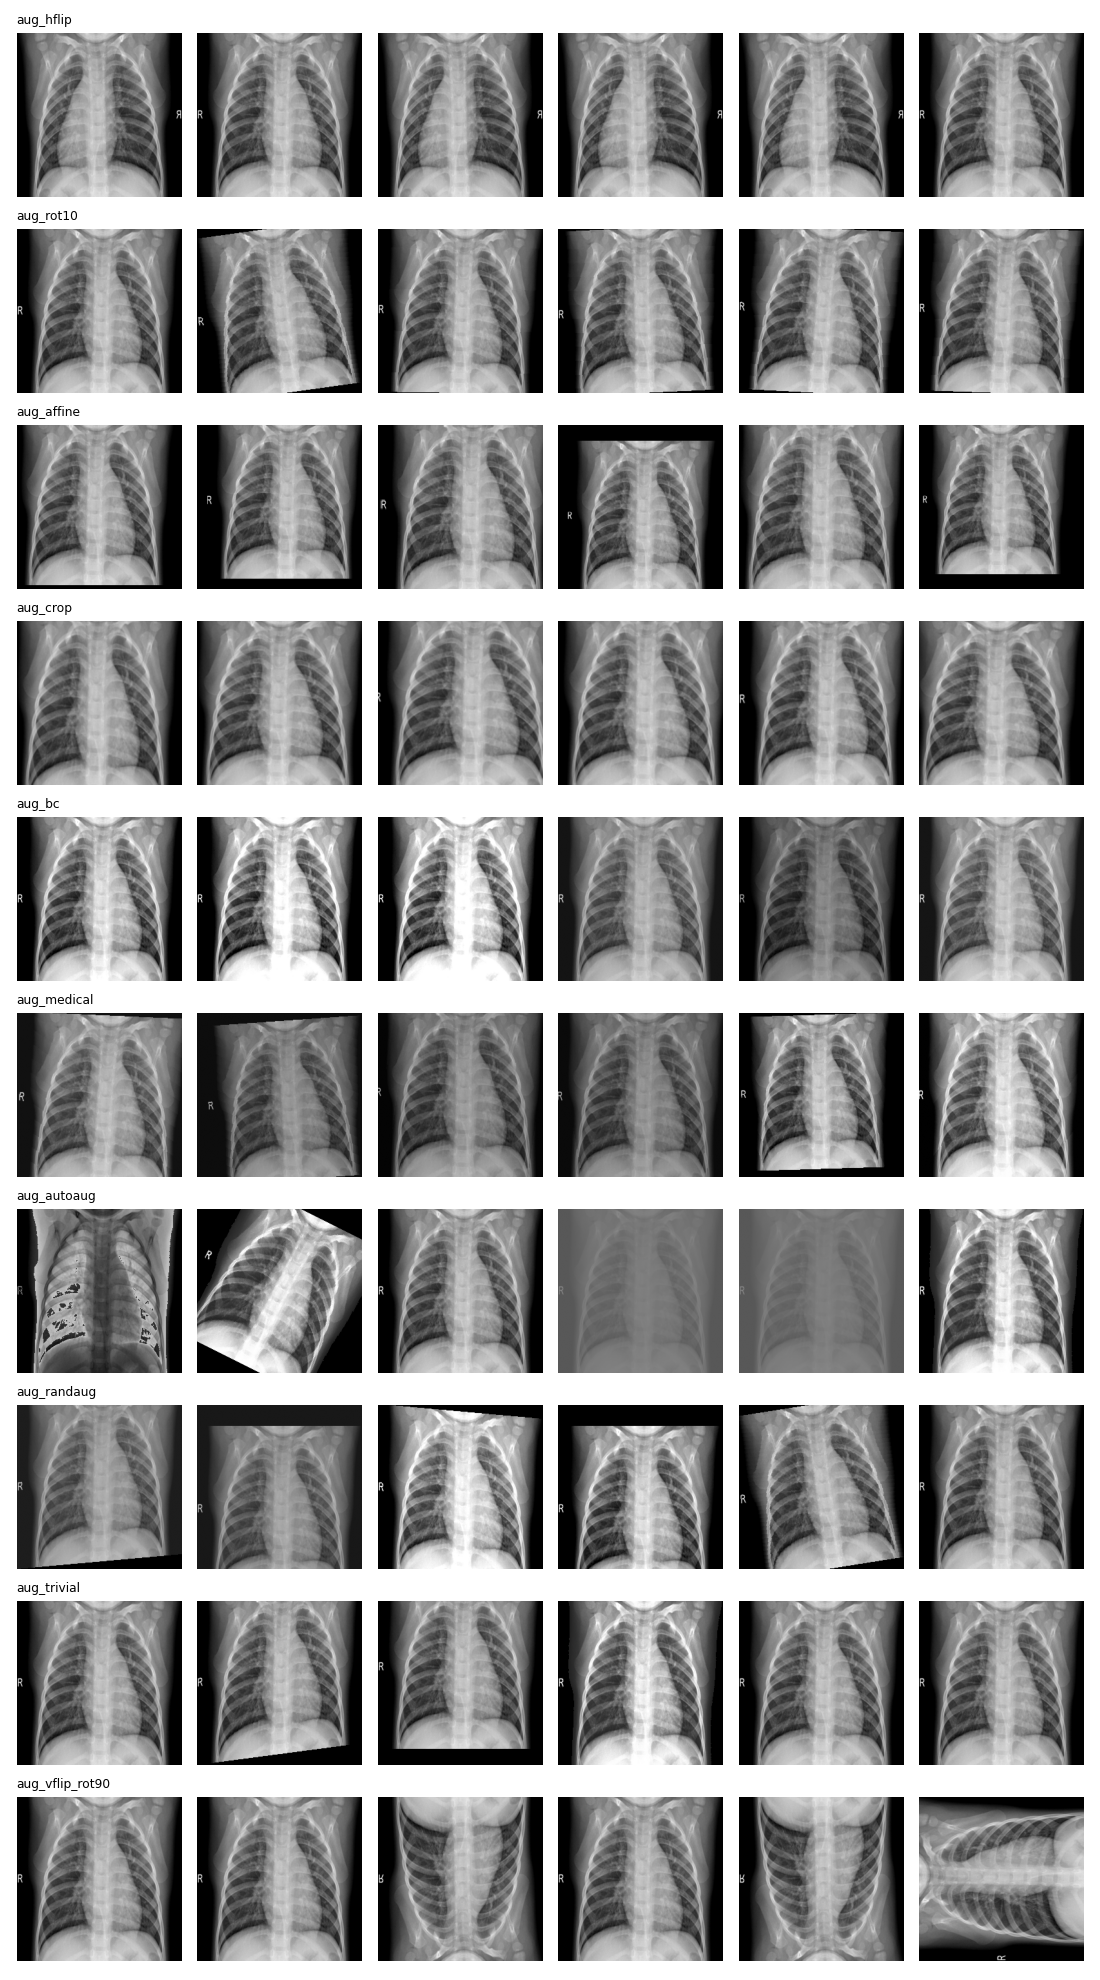
\includegraphics[width=.8\linewidth]{s5_aug_examples.png}
\caption{Six random draws of each policy on one PNEUMONIA training image.}\end{figure}
\rtab{\tabaug}{Data augmentation. \texttt{medical} = rotation $\pm7^\circ$ + translation 5\,\% + scale 0.92--1.08 + brightness/contrast 0.2. \texttt{vflip\_rot90} is an anatomically implausible control.}
\begin{figure}[H]\centering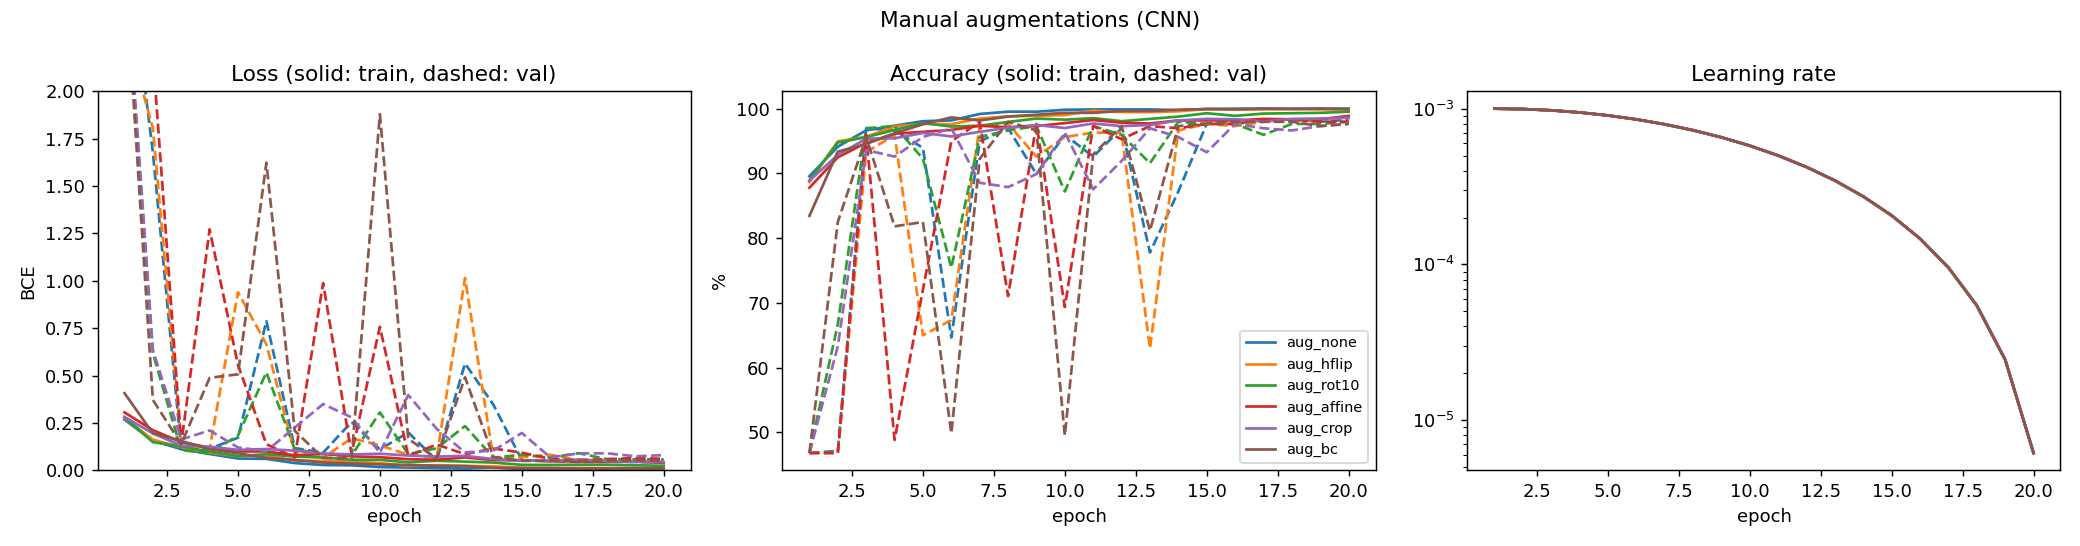
\includegraphics[width=\linewidth]{s5_manual.png}\\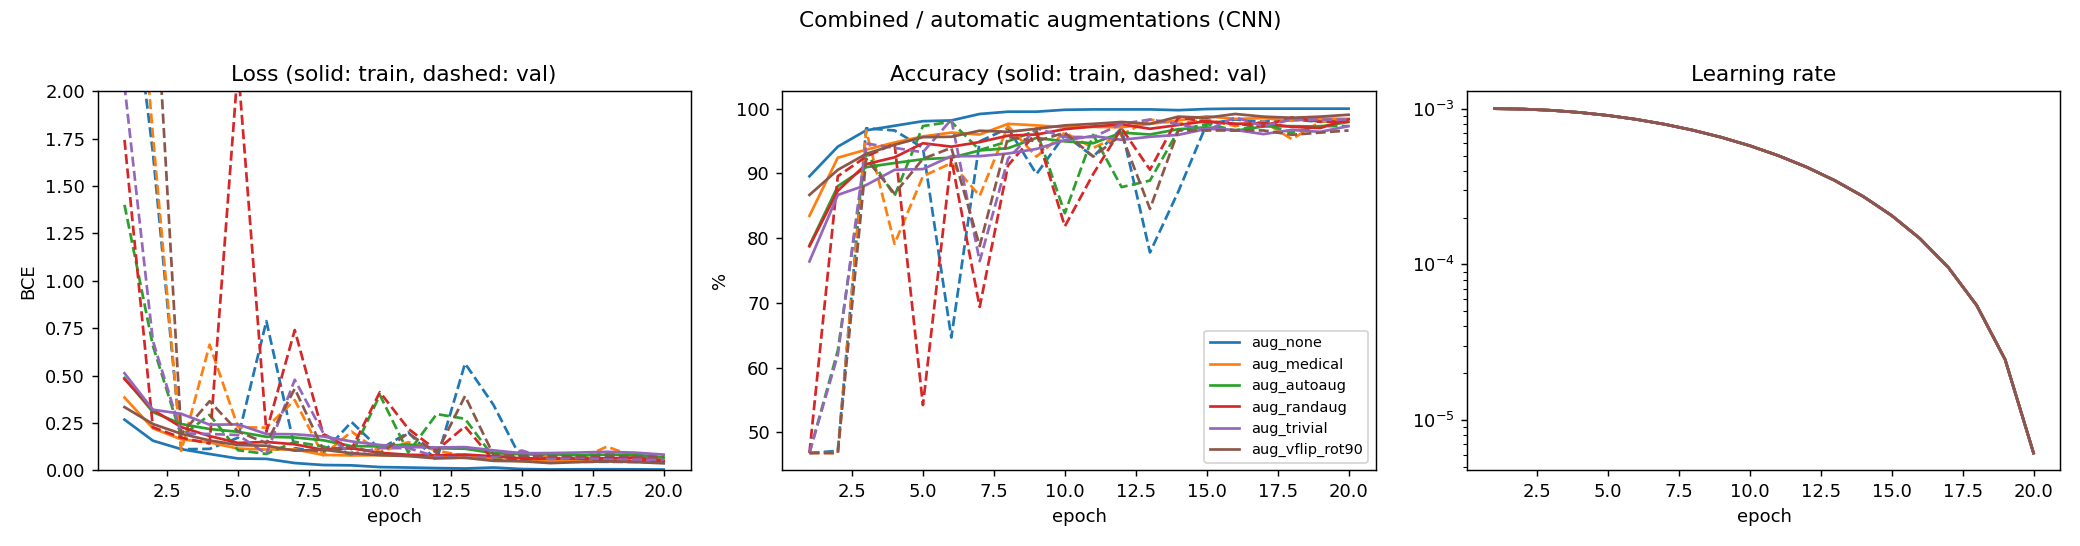
\includegraphics[width=\linewidth]{s5_auto.png}
\caption{Top: manual augmentations. Bottom: combined and automatic policies.}\end{figure}
\textbf{Effect on overfitting.} Without augmentation, the CNN reaches a training loss of 0.004 (it memorizes the training set).
All rotation, affine, crop and automatic policies keep the training loss higher (0.02--0.08) and reduce the train--val gap, so they act as regularizers.
The validation accuracy changes very little (97.6--98.7\,\% for all policies, which is a range of about 3 images).
The val-split comes from the same distribution as the training set, so it cannot show which policy helps on the shifted test set.
The test set shows clear differences.

\textbf{Which augmentations help.}
\begin{itemize}
\item \textbf{Small geometric transforms help most.} Rotation $\pm10^\circ$, affine (translation 6\,\%, scale 0.9--1.1) and mild random-resized crops raise test specificity from 51\,\% to 59--63\,\% and AUC from 94.1 to 94.7--95.9.
 Real chest radiographs differ in patient position, field of view and magnification, so these transforms simulate real variation, and the network becomes less sensitive to where the lungs are in the image.
\item \textbf{Brightness/contrast alone does not help} (test 80.8\,\%, specificity 50.9\,\%).
 The intensity differences between the sources are larger than $\pm30\,\%$ jitter, and the model can still use other shortcuts, such as position, scale and markers.
\item \textbf{The combined medical policy is the best} (rotation $\pm7^\circ$, translation, scale 0.92--1.08 and brightness/contrast 0.2): test accuracy 88.9\,\%, specificity 73.9\,\%, AUC 96.3.
 This is the best single-seed result of all experiments.
 The geometric and intensity changes together cover more of the variation between acquisitions, and every transform still gives a plausible radiograph.
\item \textbf{Automatic policies} (AutoAugment, RandAugment, TrivialAugment) also improve AUC (93.4--95.6), but less than the medical policy.
 These policies were designed for natural RGB images. They contain operations that change diagnostic information: solarize and posterize change the gray levels that encode tissue density, equalize changes the global contrast, and strong shear distorts the anatomy.
 Some of their samples are no longer realistic X-rays (see the examples figure).
 AutoAugment with the ImageNet policy has its best checkpoint at epoch 6 and the lowest AUC of the three.
\item \textbf{Flips.} A horizontal flip does not help (test 80.3\,\%, AUC 93.5).
 A chest X-ray is not left--right symmetric: the heart is on the left, and the side markers would also be mirrored. A flipped image shows anatomy that rarely occurs (dextrocardia).
 The implausible control (vertical flip + 90$^\circ$ rotation) gives the lowest validation accuracy (96.6\,\%) and no test gain. The network must learn upside-down lungs that never appear at test time, which wastes model capacity.
\end{itemize}
\textbf{Suitable for chest X-rays:} small rotations ($\le 10^\circ$), small translations and scaling, mild crops that keep both lungs in the image, and mild brightness/contrast changes.
\textbf{Not suitable:} vertical flips, large rotations, horizontal flips (questionable), solarize, posterize, inversion, color operations, and strong shear or crops that can remove the opacity that defines the label.

%==============================================================
\section{Conclusion}
\subsection{Final model}
To choose the final configuration without using the test set, I rank all experiments of Sections 1--5 by val-split accuracy and break ties by val-split loss.
\texttt{aug\_randaug}, \texttt{aug\_hflip} and \texttt{aug\_trivial} have the same validation accuracy (98.65\,\%), and RandAugment has the lowest validation loss, so it is selected.
The final model is the CNN of Section 4 with RandAugment ($N=2$, $M=9$), Adam lr $10^{-3}$, weight decay $10^{-3}$, batch size 64 and a cosine schedule.
I retrain it for 30 epochs (instead of 20) with 3 seeds, so it is not identical to the selected 20-epoch run.

\rtab{\tabfinal}{Final model, 3 seeds (30 epochs, cosine schedule).}
\begin{figure}[H]\centering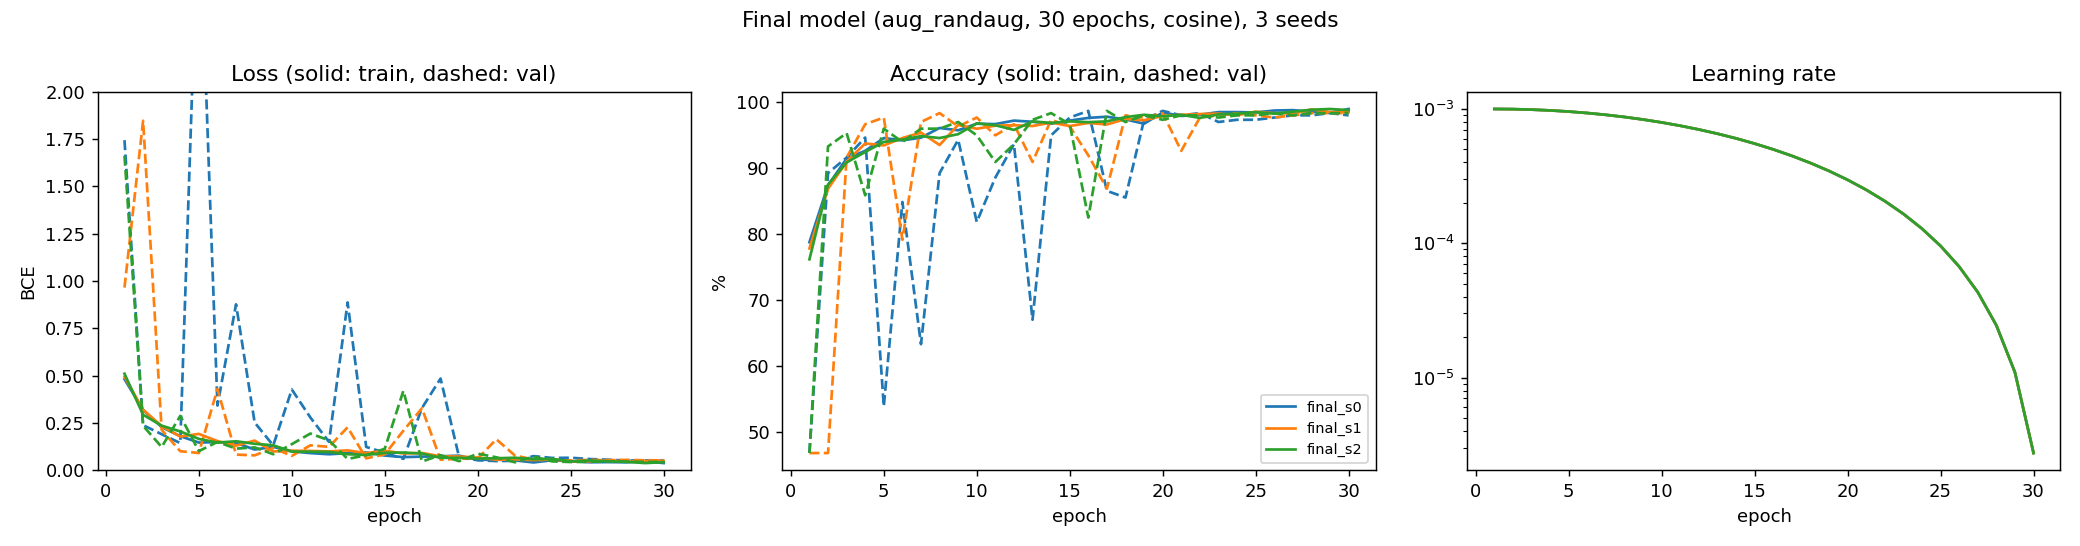
\includegraphics[width=\linewidth]{s6_final.png}\\
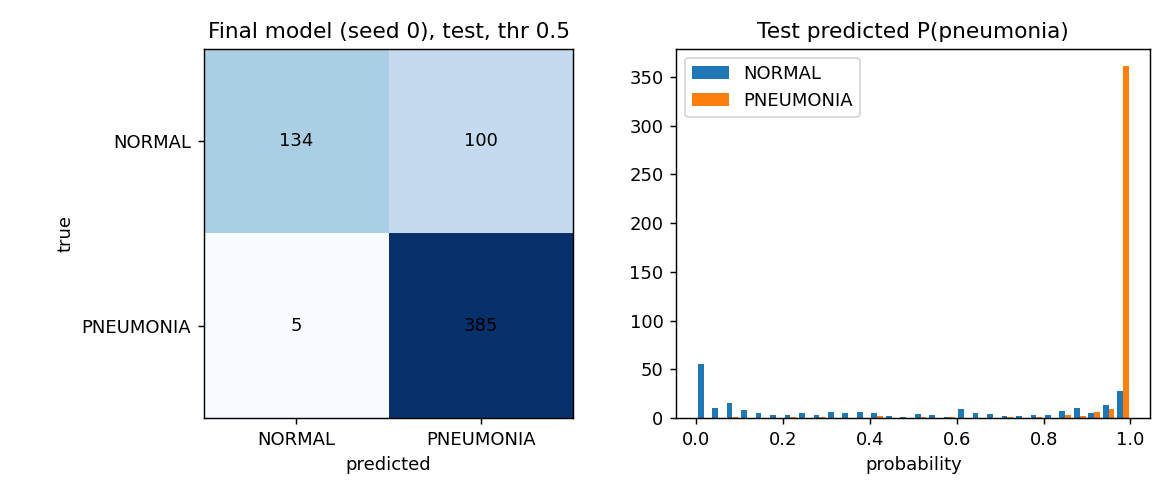
\includegraphics[width=.6\linewidth]{s6_cm.png}
\caption{Final model: learning curves of the 3 seeds; test confusion matrix (seed 0) and the distribution of the predicted probabilities.}\end{figure}

\begin{table}[H]\centering\small\caption{Test performance, mean $\pm$ std over 3 seeds (threshold 0.5).}
\begin{tabular}{lccccc}\toprule
 & val-split acc & test acc & sensitivity & specificity & AUC\\\midrule
baseline MLP (10 ep) & \basevalacc & \baseacc & \basesens & \basespec & \baseauc\\
final CNN + RandAugment (30 ep) & \finalvalacc & \finalacc & \finalsens & \finalspec & \finalauc\\
\bottomrule\end{tabular}\end{table}

\textbf{Final result.} The final model improves every test metric compared with the baseline. Test accuracy rises from \baseacc\ to \finalacc, and AUC rises from \baseauc\ to \finalauc.
The variation across seeds is also much smaller: the AUC standard deviation is 0.4 instead of 1.5.
Sensitivity is high (\finalsens), so almost no pneumonia case is missed.
The remaining errors are almost all false positives. In seed 0, 100 of the 234 NORMAL test images are predicted as PNEUMONIA, and only 5 of the 390 PNEUMONIA images are missed.
The predicted probabilities (figure above) show that the test NORMAL images spread over the whole range, while the val-split NORMAL images are separated clearly.
This again indicates a distribution shift between the training and test sources, not a lack of capacity.
I also selected a threshold by maximizing val-split accuracy. It is 0.42, and it does not help (test accuracy 82.7\,\% vs.\ 83.2\,\%), because the val-split is too easy to show the shift.
The best single run of the study (\texttt{aug\_medical}: 88.9\,\% / AUC 96.3) was not selected by the validation rule. Section 6.3 discusses this.

\subsection{Summary of all experiments}
Tables 2--11 list every run. Table~\ref{tab:summary} collects the most informative run of each section. The main observations are below, ordered from the largest effect to the smallest:
\begin{table}[H]\centering\small\caption{Summary: key runs of every section (seed 0 unless named \texttt{final\_s}$k$).}\label{tab:summary}\begin{tabular}{lrrrrrrrrr}\toprule\thead \tabsummary \bottomrule\end{tabular}\end{table}
\begin{enumerate}
\item \textbf{The validation protocol has the largest effect on the conclusions.} The official 16-image validation set cannot separate the models (its accuracy ranges from 62.5 to 100\,\% across models whose test scores are similar).
  A patient-grouped val-split of 297 images is necessary for meaningful checkpoint and model selection.
\item \textbf{Architecture (CNN vs.\ MLP).} The CNN improves validation accuracy (96 $\rightarrow$ 98\,\%), validation loss (0.11 $\rightarrow$ 0.04) and test AUC (about 91.5 $\rightarrow$ 94), with 17 times fewer parameters.
\item \textbf{Data augmentation that matches real variation.} Small geometric changes, combined with mild intensity changes, are the only factor that clearly improves test specificity, from about 51\,\% to 74\,\% for the best policy.
  This is the factor that addresses the train/test distribution shift.
\item \textbf{Optimization and schedule} decide whether training converges and stays stable. lr $10^{-2}$, plain SGD and batch size 256 are slower or unstable, and a decaying schedule removes the late oscillations.
  However, once training converges and the checkpoint is selected, these factors change the test result by less than the seed noise.
\item \textbf{Small effects:} weight decay between 0 and $10^{-2}$, MLP depth and width, CNN width, and CNN dropout.
\end{enumerate}

\subsection{Limitations and possible improvements}
\begin{itemize}
\item \textbf{Single seed.} Except for the baseline and the final model, each run uses one seed. The seed standard deviation of the baseline (about 3 points of test accuracy, more than 10 points of specificity) is larger than most of the differences in Sections 2--4.
  A stronger study would run 3--5 seeds per configuration and report confidence intervals.
\item \textbf{The model selection does not measure robustness to distribution shift.} The val-split comes from the training distribution and is saturated (97.6--98.7\,\% for all CNN runs, a range of 3 images).
  For this reason, the selection rule chose RandAugment and not the medical policy, although the medical policy has clearly better test specificity.
  A validation set from the test-like source would be better (for example a held-out hospital or acquisition batch), or k-fold cross-validation with more data.
\item \textbf{Threshold and calibration.} The training set is balanced and the test set is 62.5\,\% PNEUMONIA, and the test errors are mostly false positives. A decision threshold chosen on data that represents the deployment setting, or probability calibration, would trade some sensitivity for specificity in a controlled way.
\item \textbf{Compute.} All runs used a CPU, so the CNN is small and trained for 20--30 epochs, and no pretrained models were used. ImageNet-pretrained ResNet or DenseNet fine-tuning, higher resolution, and longer training would probably improve the robustness.
\item \textbf{Data.} The subset uses 2000 of the about 5200 original training images. Patient IDs are only reliable within one official split.
  A more careful study would also check the shortcut features (for example the ``R'' marker and the border) with saliency maps.
\end{itemize}
\end{document}
